%% ut-thesis.tex -- document template for graduate theses at UofT
%%
%% Copyright (c) 1998-2012 Francois Pitt <fpitt@cs.utoronto.ca>
%% last updated at 09:43 (EDT) on Fri  1 Jun 2012
%%
%% This work may be distributed and/or modified under the conditions of
%% the LaTeX Project Public License, either version 1.3c of this license
%% or (at your option) any later version.
%% The latest version of this license is in
%%     http://www.latex-project.org/lppl.txt
%% and version 1.3c or later is part of all distributions of LaTeX
%% version 2005/12/01 or later.
%%
%% This work has the LPPL maintenance status "maintained".
%%
%% The Current Maintainer of this work is
%% Francois Pitt <fpitt@cs.utoronto.ca>.
%%
%% This work consists of the files listed in the accompanying README.

%% SUMMARY OF FEATURES:
%%
%% All environments, commands, and options provided by the `ut-thesis'
%% class will be described below, at the point where they should appear
%% in the document.  See the file `ut-thesis.cls' for more details.
%%
%% To explicitly set the pagestyle of any blank page inserted with
%% \cleardoublepage, use one of \clearemptydoublepage,
%% \clearplaindoublepage, \clearthesisdoublepage, or
%% \clearstandarddoublepage (to use the style currently in effect).
%%
%% For single-spaced quotes or quotations, use the `longquote' and
%% `longquotation' environments.


%%%%%%%%%%%%         PREAMBLE         %%%%%%%%%%%%

%%  - Default settings format a final copy (single-sided, normal
%%    margins, one-and-a-half-spaced with single-spaced notes).
%%  - For a rough copy (double-sided, normal margins, double-spaced,
%%    with the word "DRAFT" printed at each corner of every page), use
%%    the `draft' option.
%%  - The default global line spacing can be changed with one of the
%%    options `singlespaced', `onehalfspaced', or `doublespaced'.
%%  - Footnotes and marginal notes are all single-spaced by default, but
%%    can be made to have the same spacing as the rest of the document
%%    by using the option `standardspacednotes'.
%%  - The size of the margins can be changed with one of the options:
%%     . `narrowmargins' (1 1/4" left, 3/4" others),
%%     . `normalmargins' (1 1/4" left, 1" others),
%%     . `widemargins' (1 1/4" all),
%%     . `extrawidemargins' (1 1/2" all).
%%  - The pagestyle of "cleared" pages (empty pages inserted in
%%    two-sided documents to put the next page on the right-hand side)
%%    can be set with one of the options `cleardoublepagestyleempty',
%%    `cleardoublepagestyleplain', or `cleardoublepagestylestandard'.
%%  - Any other standard option for the `report' document class can be
%%    used to override the default or draft settings (such as `10pt',
%%    `11pt', `12pt'), and standard LaTeX packages can be used to
%%    further customize the layout and/or formatting of the document.

%% *** Add any desired options. ***
\documentclass{ut-thesis}

%% *** Add \usepackage declarations here. ***
%% The standard packages `geometry' and `setspace' are already loaded by
%% `ut-thesis' -- see their documentation for details of the features
%% they provide.  In particular, you may use the \geometry command here
%% to adjust the margins if none of the ut-thesis options are suitable
%% (see the `geometry' package for details).  You may also use the
%% \setstretch command to set the line spacing to a value other than
%% single, one-and-a-half, or double spaced (see the `setspace' package
%% for details).


%%%%%%%%%%%%%%%%%%%%%%%%%%%%%%%%%%%%%%%%%%%%%%%%%%%%%%%%%%%%%%%%%%%%%%%%
%%                                                                    %%
%%                   ***   I M P O R T A N T   ***                    %%
%%                                                                    %%
%%  Fill in the following fields with the required information:       %%
%%   - \degree{...}       name of the degree obtained                 %%
%%   - \department{...}   name of the graduate department             %%
%%   - \gradyear{...}     year of graduation                          %%
%%   - \author{...}       name of the author                          %%
%%   - \title{...}        title of the thesis                         %%
%%%%%%%%%%%%%%%%%%%%%%%%%%%%%%%%%%%%%%%%%%%%%%%%%%%%%%%%%%%%%%%%%%%%%%%%

%% *** Change this example to appropriate values. ***
\degree{Master of Science}
\department{Computer Science}
\gradyear{2015}
\author{Priya Sidhaye}
\title{Parameterized Text Summarization}

%% *** NOTE ***
%% Put here all other formatting commands that belong in the preamble.
%% In particular, you should put all of your \newcommand's,
%% \newenvironment's, \newtheorem's, etc. (in other words, all the
%% global definitions that you will need throughout your thesis) in a
%% separate file and use "\input{filename}" to input it here.


%% *** Adjust the following settings as desired. ***

%% List only down to subsections in the table of contents;
%% 0=chapter, 1=section, 2=subsection, 3=subsubsection, etc.
\setcounter{tocdepth}{2}

%% Make each page fill up the entire page.
\flushbottom


%%%%%%%%%%%%      MAIN  DOCUMENT      %%%%%%%%%%%%

\begin{document}

%% This sets the page style and numbering for preliminary sections.
\begin{preliminary}

%% This generates the title page from the information given above.
\maketitle

%% There should be NOTHING between the title page and abstract.
%% However, if your document is two-sided and you want the abstract
%% _not_ to appear on the back of the title page, then uncomment the
%% following line.
%\cleardoublepage

%% This generates the abstract page, with the line spacing adjusted
%% according to SGS guidelines.
\begin{abstract}
%% *** Put your Abstract here. ***
%% (At most 150 words for M.Sc. or 350 words for Ph.D.)
\end{abstract}

%% Anything placed between the abstract and table of contents will
%% appear on a separate page since the abstract ends with \newpage and
%% the table of contents starts with \clearpage.  Use \cleardoublepage
%% for anything that you want to appear on a right-hand page.

%% This generates a "dedication" section, if needed
%% (uncomment to have it appear in the document).
%\begin{dedication}
%% *** Put your Dedication here. ***
%\end{dedication}

%% The `dedication' and `acknowledgements' sections do not create new
%% pages so if you want the two sections to appear on separate pages,
%% you should put an explicit \newpage between them.

%% This generates an "acknowledgements" section, if needed
%% (uncomment to have it appear in the document).
%\begin{acknowledgements}
%% *** Put your Acknowledgements here. ***
%\end{acknowledgements}

%% This generates the Table of Contents (on a separate page).
\tableofcontents

%% This generates the List of Tables (on a separate page), if needed
%% (uncomment to have it appear in the document).
%\listoftables

%% This generates the List of Figures (on a separate page), if needed
%% (uncomment to have it appear in the document).
%\listoffigures

%% You can add commands here to generate any other material that belongs
%% in the head matter (for example, List of Plates, Index of Symbols, or
%% List of Appendices).

%% End of the preliminary sections: reset page style and numbering.
\end{preliminary}


%%%%%%%%%%%%%%%%%%%%%%%%%%%%%%%%%%%%%%%%%%%%%%%%%%%%%%%%%%%%%%%%%%%%%%%%
%%  Put your Chapters here; the easiest way to do this is to keep     %%
%%  each chapter in a separate file and `\include' all the files.     %%
%%  Each chapter file should start with "\chapter{ChapterName}".      %%
%%  Note that using `\include' instead of `\input' will make each     %%
%%  chapter start on a new page, and allow you to format only parts   %%
%%  of your thesis at a time by using `\includeonly'.                 %%
%%%%%%%%%%%%%%%%%%%%%%%%%%%%%%%%%%%%%%%%%%%%%%%%%%%%%%%%%%%%%%%%%%%%%%%%

%% *** Include chapter files here. ***
\chapter{Introduction}

Natural Language Generation is the process of generating human-readable texts. The generation system can take as an input another text itself, or some internal representation of data. Language generation has been used in systems for a long time in order to communicate information, ranging from a report generation to small text generation. One of the first successful generation systems used weather data to generate a report in the form of a daily weather update. 

Another type of generation systems take text as input, to produce a different kind of text. This kind of generation is called text-to-text generation. Summarization of text is an excellent example of text-to-text generation. The problem we look at during the course of this research is text-to-text generation between different genres of texts.
\chapter{Background and Related Work}
\label{chap:background}

This chapter contains the literature survey and the background for the thesis. Background on various concepts used in the thesis alongwith numerous related studies, especially on Twitter data are then discussed.


\section{Summarization}

Summarization is the task of condensing the original text document while retaining as much of the important information as possible. Other goals include readability of the generated summary and coherence. The two main approaches for automatic text summarization are \textit{extractive} and \textit{abstractive} summarization. Extractive summarization uses the technique of extract and rearrange. \cite{nenkova2012survey} describe the components in extractive summarization techniques as building an internal representation of the important parts of the text, ranking these in the order of importance/time etc and then selecting a suitable list of these sentences to eventually form the summary. In phrase-level summarization, smoothing techniques may be used to generate readable texts. Sentence-level summarization techniques tend do be inherently more cohesive since sentences are directly picked out, however, sentence compression techniques can be used to reduce the size of the summaries. Even after using smoothing techniques to generate readable text, the summaries tend to be incoherent and hard to read. \figref{fig:extractive} shows an example of extractive summarization where a couple of sentences from the article have been picked to show in the the thumbnail for an article.

\begin{figure}[!htbp]
\centering
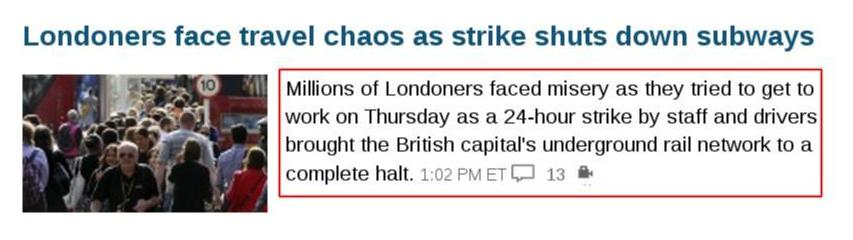
\includegraphics[width=\textwidth, height=4.5cm]{extractive}
\caption{Example of extractive summarization.}
\label{fig:extractive}
\end{figure}


The second approach is that of abstractive summarization. This is a text-to-text generation approach that aims at keeping the content or meaning of the text the same while condensing the text or generalizing it. As a rule, abstractive summarization requires world knowledge and is a much more difficult problem to solve. In fact, it is a rather large challenge and current summarization techniques concentrate on improving results from extractive summarization. \figref{fig:abstractive} shows the same thumbnail for a news article. However, the title of the article is an abstractive summary that is a generalization of the events described, carefully omitting details yet leaving the overall meaning of the event untouched.

\begin{figure}[!htbp]
\centering
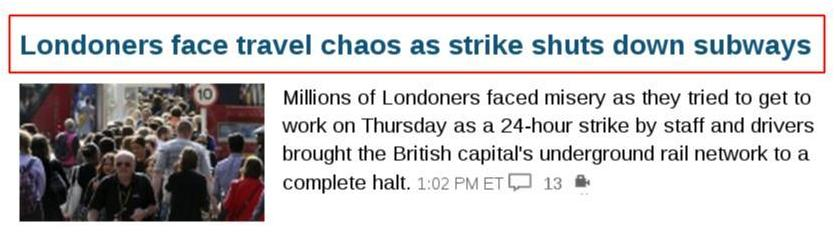
\includegraphics[width=\textwidth, height=4.5cm]{abstractive}
\caption{Example of abstractive summarization.}
\label{fig:abstractive}
\end{figure}

The limits of extractive summarization have been studied by \cite{he2000comparing}. They compare user preferences for various types of summaries of an audio-visual presentation. They demonstrate that the most preferred method of summarization is highlights and notes provided by the author, rather than transcripts or slides from the presentation. \cite{conroy2006topic} computed an oracle ROUGE score to investigate the same issue of the limits of extraction for news text. The oracle score is based on the maximum likelihood probability of words occurring in model summaries and is in turn used to generate summaries that perform better than any extracted and also human-generated summaries.

\subsection{ROUGE: Evaluation measure for Text Summarization}

ROUGE is an evaluation measure popularly used for evaluating quality of summaries and was proposed by \cite{lin-2004}. It measures the quality of the summary by comparing the output of the system being tested against a set of gold standard summaries. The intuition is that if the generated summary has enough in common with a set of human-written summaries, then it can be judged as a good summary. The different types of comparisons calculated are the unigram, bigram, trigram and least common subsequence(ROUGE-1,2,3 and L respectively). A set of gold standard summaries are used to encompass the number of possibilities while generating summaries. 

\begin{equation}
ROUGE-N = \frac{\sum\limits_{S \in \{Reference Summaries\}} \sum\limits_{gram_n \in S} Count_{match}(gram_n)}{\sum\limits_{S \in \{Reference Summaries\}} \sum\limits_{gram_n \in S} Count(gram_n)}
\end{equation}

The equation as described by \cite{lin2004looking} shows the calculation of the ROUGE-N score, where $n$ is the length of the n-gram, and $Count_{match}$ is the length of the matched n-grams in the summary and the reference summaries.

The use of multiple gold standard summaries gives rise to a subjective evaluation metric where the quality of the evaluation is dependent on the quality and number of the gold standard summaries. ROUGE also does not calculate take into account whether the summary is fluent or coherent. However, it is useful in the extractive text summarization systems where content retention needs to be judged since it uses n-gram co-occurrence statistics.

% \section{Stylistics}
%\change{remove this and put it in the formality part}
% Stylistics is referred to the characteristics of text that can be extracted from it that do not relate to the meaning of the text. Common examples of these include textual statistics such as length of sentences and words, parts of speech, function words etc. and finds applications in authorship attribution, semantic analysis, personality typing and so on. Studies on building lexicons for formality have been conducted and are discussed further later \chapref{chap:analysis}.

\section{Studies based on Twitter data}

There have been studies on a number of different issues related to Twitter data, including classifying tweets and sentiment analysis of tweets. \cite{ghosh2011entropy} classified the retweeting activity of users based on time intervals between retweets of a single user and frequency of retweets from unique users. 'Retweet' here means the occurrence of the same URL in a different tweet. The study was able to classify the retweeting as automatic or robotic retweeting, campaigns, news, blogs and so on, based on the time-interval and user-frequency distributions. In another study, \cite{chen2012extracting} were able to extract sentiment expressions from a corpus of tweets including both formal words and informal slang that bear sentiment.

Other studies using Twitter data include \cite{o2010tweetmotif}, who use topic summarization for a given search for better browsing. \cite{chakrabarti2011event} generate an event summary by learning about the event using a Hidden Markov Model over the tweets describing it. \cite{wang2014socially} generate a coherent event summary by treating summarization as an optimization problem for topic cohesion. \cite{inouye2011comparing} compare multiple summarization techniques to generate a summary of multi-post blogs on Twitter. \cite{wei2014utilizing} use tweets to help in generating better summaries of news articles.

% detailed analysis of this paper
As described in \chapref{chap:intro}, we analyze tweet generation using measures inspired by extractive summarization evaluation. There has been one study comparing different text summarization techniques for tweet generation by \cite{lloret2013towards}. Summarization systems were used to generate sentences lesser than 140 characters in length by summarizing documents, which could then be taken to be tweets. The system-generated tweets were evaluated using ROUGE measures \cite{lin2004rouge}. The ROUGE-1, ROUGE-2 and ROUGE-L measures were used, and a human-written reference tweet was taken to be the gold standard. %ROUGE has been known to work better when multiple reference summaries are used and is not meant to be used at the sentence level. This study uses ROUGE with a single reference summary, which is the reference tweet. However, given the size of a tweet, it can be argued that while generating a reference tweet from a single document, it is difficult to generate multiple reference tweets with largely varying content. \unsure{Is this reasoning okay?}

These studies show that extractive summarization algorithms may not generate good quality summaries despite giving high ROUGE evaluation scores. \cite{cheung2013towards} show that for the news genre, extractive summarization systems that are optimized for \textit{centrality}---that is, getting the core parts of the text into the summary---cannot perform well when compared to model summaries, since the model summaries are abstracted from the document to a large extent.

\chapter{Data Extraction}

Data was extracted from Twitter using the Twitter REST API using 51 search terms, or ‘hashtags’. These hashtags were chosen from a range of topics including pop culture,  international summit meetings discussing political issues, lawsuits and trials, social issues and health care issues like the recent outbreak of ebola. All these hashtags were ‘trending’ (being tweeted about at a high rate) at the time of extraction of the data. To give the data some variety, the data was extracted over the course of 15 days, which gave us multiple news stories to choose from for the search terms. Only English tweets were extracted since the study is limited to English. In the beginning, about 30,000 tweets were extracted, and more than half of these tweets, around 16,000 contained URLs referencing some news articles, photos on photo sharing sites, and videos. The hashtags were chosen to maximise the number of articles related to the tweets. Hence, a lot of topics that were chosen were being tweeted about by news agencies and other popular news sources.

The articles referenced by the tweets were extracted using the URLs mentioned in the tweets. The ‘newspaper’ package was used to extract article text and the title from the web page.
\chapter {Preprocessing}

The data from the tweets was cleaned by removing the tweets that were in different languages as well as the ones that were retweeted, which is equivalent of re-publishing the same tweet from a different user. 

Unique URLs were first extracted from the 16,000 or so URLs in the data. Next, data from these unique URLs was extracted and then preprocessed. For the articles obtained from URLs, photos and video links for example, from Instagram and Youtube needed to be removed. For this, the data cleaning was achieved by removing articles by limiting word length of the extracted text to about 150 words. This ensured the removal of photos, videos, advertisements, incorrectly extracted articles from the data.  After this preprocessing, the number of useful articles reduced to 3066 from 6003.

\section {Tagging articles}

For the first trial for tagging, a sample set of 100 articles were tagged by two people. The tags used in the preliminary tags were : ‘evaluative’ vs ‘descriptive’ and ‘traditional’ vs ‘nontraditional’ news sources. ‘Evaluative’ text is a more opinionated text, that is more subjective. This text will be expected to take a certain object or event, analyze it,  and form an opinion about it. ‘Descriptive’ text is non-evaluative, containing for example a narration of an event or an explanation about a certain object or event. A ‘mixed’ category was also added to accommodate some in-between articles. ‘Traditional’ texts are the ones published by established news houses and a more formal form of discourse. ‘Nontraditional’ texts are a more colloquial and informal way of writing text - longer, with less fact verification and a more explanatory and narrative kind of feel to it. These also include shorter web articles that are somewhere between a blog post and a news article. They are not as free of rules as a blog post, but are not in the style of a rigid news article.

The title, the text and origin of the articles were considered while tagging them. The tagging itself was subjective based on the opinion of the tagger about what category the article fell into. It was observed that there were a few judgement calls, specially between the evaluative/descriptive/mixed tags.

Correlation was calculated between the two different sets of tags to check if the opinions about the articles were unanimous. The Cohen’s kappa value was used for the purpose. Overall, the kappa value turned out to be 0.69. However, it was found that there was high correlation between the taggers for traditional vs. nontraditional texts with a kappa value of 0.88, and lesser correlation for evaluative/descriptive/mixed texts, 0.13. This seems to suggest an absence of an exact definition of evaluative versus descriptive texts. 

However, the Cohen’s kappa value shows that traditional vs nontraditional tags correlate well between taggers. Upon analysis of the ones that differed, the differences of opinions between the taggers could be resolved. This suggests that, this axis of description for the article as traditional vs nontraditional can be tagged accordingly.

\section {Current description of data}

The data currently consists of all tweets alongwith all the information of the tweet itself, such as the text of the tweet, links to articles if any, hashtags, and so on. The article links from these tweets are stored as a separate file, with information about the articles themselves, along with some preprocessed data. This includes the URL itself and the text extracted from the article, as well as some extracted information such as sentence boundaries, POS tags for tokens, parse trees and dependency trees. This processing of the text was done using the CoreNLP toolkit developed at Stanford (Manning et al., 2014 \cite{manning2014stanford})

Tweets are linked to URLs through another file. A URL could have been tweeted through multiple tweets, all the ids of these tweets are linked to the same URL. 

\chapter {Experiments}

\section {Subjectivity and Formality }

After tagging a sample set of articles, the natural next task was to determine if the articles could be tagged automatically based on characteristics of the text. To achieve this, the degree of subjectivity and formality of the text was calculated with the help of some other studies. The subjectivity lexicon (Wilson et al., 2005 \cite{wilson2005recognizing}) was built using data for subjectivity analysis for a given text. The subjectivity lexicon consists of words that might indicate an opinion being expressed in a given text. Similarly, the formality lexicon gives was generated by Brooke et al. 2013 \cite{brooke2013multi} and can be used to measure formality of a given text. The lexicon consists of words and phrases and the degree of formality for their occurrence. Thus, more formal words marked on a positive scale and informal words like those occurring in colloquial language are marked on a negative scale. Using the formality and subjectivity lexicons, the degree of subjectivity and formality of each individual article was calculated. 

The degree of subjectivity returned a count per of the number of words present in the article that suggested an opinion per article. This number was normalized with the length of the article, and the degree of subjectivity was calculated per 10 words of an article. For this result, only the strong subjective entries in the lexicon were used to better differentiate between subjective and non-subjective articles.

The formality lexicon gave positive weights for formal expressions and negative for informal expressions. After calculating the formality weights for all articles, it was observed that they all had a total negative normalized weight, meaning a lot more informal expressions were getting matched. Hence, we used just the formal word occurrences for calculating the weight. Thus, above a certain cut-off weight, the article could be considered formal, else would be considered informal.

All the weights from both lexicons were averaged out over the articles relating to a single search term(or hashtag), and then ranked accordingly. The ranking showed that for subjectivity ranking over hashtags, films and music related hashtags are at the top, which would be the natural intuition given the nature of the topics. On the other hand, in the formality ranking, the hashtags relating to political issues had the highest formality ranking, while the hashtags for film titles, pop culture are all at the bottom. This also correlates with intuition about the topics. As a sanity check, we also looked at articles at the extreme points of the both the graphs. The texts of these articles suggested that they were consistent with the numbers.

Correlation between the rankings of hashtags given by both these experiments was calculated, and the Kendall’s tau for this was 0.09 with a p-value of 0.34. The low correlation suggests that these two ways of evaluating subjectivity and formality are independent. The p-value suggests that there is not enough evidence to prove a correlation between subjectivity and formality of an article.

\section{Correlating descriptive/non-descriptive with formal vs. informal for automatic tagging}

To check if the descriptive vs non-descriptive tags correlated when tagged using the formality lexicon. If the document contained no formal words from the lexicon, it was tagged as non-traditional, else, it was tagged as traditional. The sample set of articles was tagged using this method, and after comparing them with the human tags, 42 out of the 62 tags matched, which gave a match percentage of 67%.

\section{Position of tweet text in article experiments}
\subsection {Total match with text in article}

We calculated the position of tweet text as a whole in the text. To compare the text, we removed the hashtags, references (@) and urls from the tweets. After this, we did direct substring comparison of the tweet in the text. 

Out of the 6144 instances where a tweet text was checked against the text in the article, a complete match was found around 70 times. 30 times out of these, the tweet text had been matched against the title of the article extracted into the text. The rest of the results are significant, since the text of the tweet appears exactly as is inside the text of the article. The user who wrote the tweet for these articles went through the article text, and the sentence that either seemed to be the most conclusive contribution of the article, or expressed the opinion of the user were extracted to be tweeted. 

We also checked to see if the tweet text matched a lot with the article titles, and this was found not to be the case. (*Needs to be verified)

\subsection{Percentage match}

Next, we did a percentage match with the text of the article after removing the stop words from both the tweet and the text. The results we got seem to suggest that a lot of significant words in the tweet are in fact present in the article. The minimum percentage match obtained was 60%.

\subsection{Percentage matching inside a window in the article text}

The next analysis was to check for a significant word matching inside a two or three sentence window inside the article text. We used a three sentence long window using the sentence boundary information obtained during preprocessing. After the text of the window was extracted, we performed a similar analysis as the last one, except on a smaller text. Next, the matching percentages from all such windows in the articles were compared and the maximum out of these was considered for the highest match percentage and match position for the final results. The final results are being verified, including the result for where the tweet text mostly comes from is random.

\subsection{Least Common Subsequence match inside a window for the text}

The percentage matched have mostly been a bag-of-words approach. The next step would be to look for phrases in the tweet coming directly from the text.

\chapter {Future Experiments}

Towards the aim of generating parameterized summarization, the next step would be to manually generate summaries for a few articles that vary according to the parameters described in the text, and perform analyses on these generated summaries and see how similar/different they are to the original text.

It would also be interesting to first manually generate tweets from articles that vary in sentiment from a given subjective text, and see how this is achieved by picking out sentences with particular sentences from the article and using it to convey the sentiment given in the parameters. For example for a review of an object, picking out a sentence describing a negative feature for a negative sentiment in the parameter.


%% This adds a line for the Bibliography in the Table of Contents.
\addcontentsline{toc}{chapter}{Bibliography}
%% *** Set the bibliography style. ***
%% (change according to your preference/requirements)
\bibliographystyle{plain}
%% *** Set the bibliography file. ***
%% ("thesis.bib" by default; change as needed)
\bibliography{thesis}

%% *** NOTE ***
%% If you don't use bibliography files, comment out the previous line
%% and use \begin{thebibliography}...\end{thebibliography}.  (In that
%% case, you should probably put the bibliography in a separate file and
%% `\include' or `\input' it here).

\end{document}
